\begin{frame}{Eigenschaften Embedded System\hcite{embeddedSpecials}}
	\pause
	\begin{multicols}{2}
		\begin{itemize}
			\item Kosten
			\item Grösse
			\item Energie
			\item Zuverlässigkeit
			\item Sicherheit
			\item Langlebigkeit
			\item Echtzeit
		\end{itemize}
	\end{multicols}
\end{frame}

\begin{frame}{Definition Embedded System}
	Der Ausdruck embedded system bezeichnet einen Computer, der in einem technischen Kontext eingebettet ist. \hcite{wikiEmbedded}
	\begin{flushright}
		Nach Wikipedia
	\end{flushright}
\end{frame}

\begin{frame}{Grösse von Embedded Systemen}
	\begin{center}
		\footnotesize{
			\begin{tabular}{p{5cm}p{5cm}}
				\only<handout>{
					Digitales Multimeter & ATLAS/LHC/CERN \\
				}
				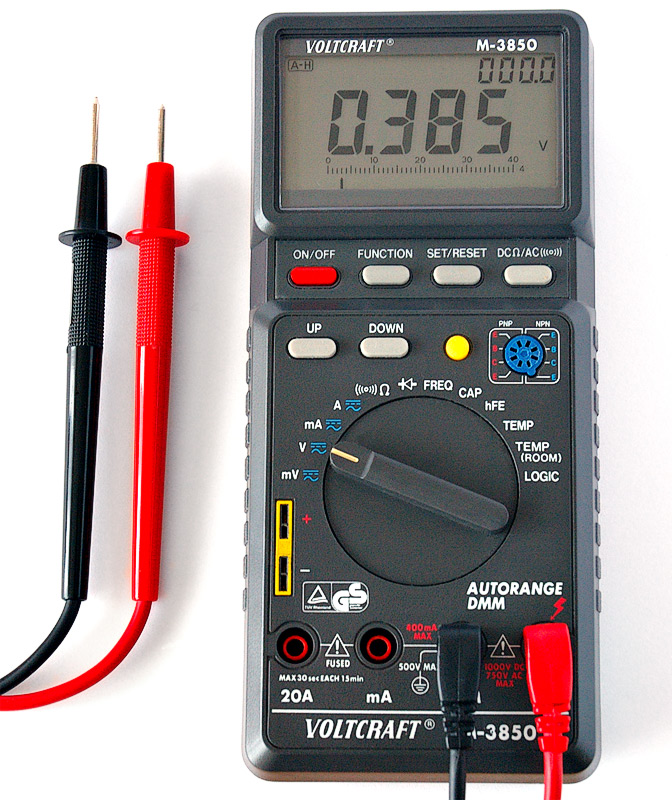
\includegraphics[height=4cm]{res/Digital_Multimeter_Aka.jpg}\hcite{multimeter} &
				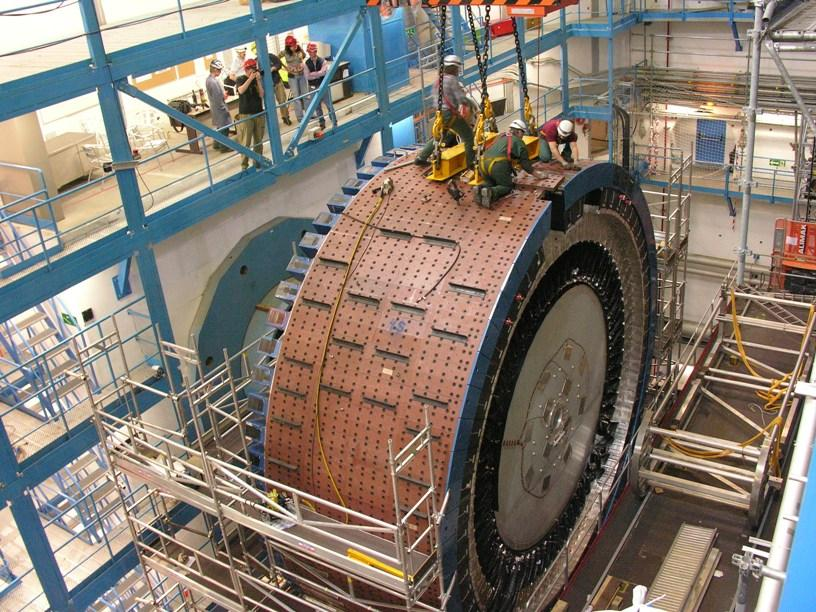
\includegraphics[height=4cm]{res/ATLAS_Tile_Calorimeter}\hcite{tileCalorimeter} \\
				\only<handout>{
					Sensor produziert ~20 B/sec & Sensor produziert 1 PiB/sec \\
					Reduzierung auf ~2 B/sec & Reduzierung auf ~100 MiB/sec \hcite{wikiAtlas}\\
					Verarbeitung auf internem uC & Verarbeitung auf eigenen 20'000 Server und Grid \hcite{wikiCernServer}
				}
			\end{tabular}
		}
	\end{center}
\end{frame}

\begin{frame}{Typisches GNU/Linux Embedded System}
	\begin{center}
		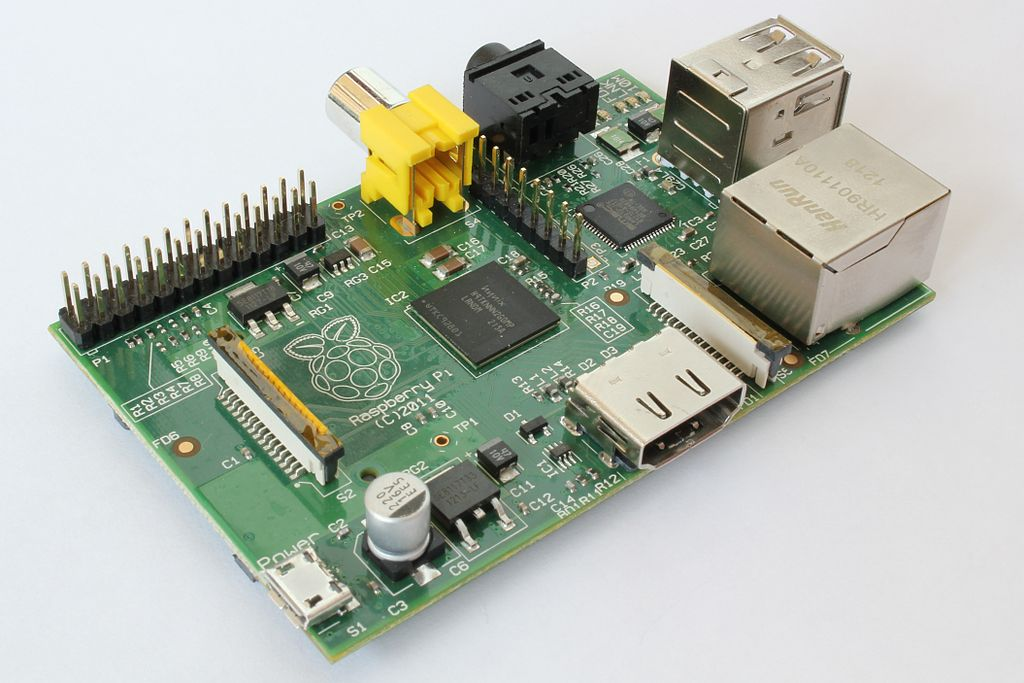
\includegraphics[width=5cm]{res/RaspberryPi.jpg}\hcite{raspberryPi}
		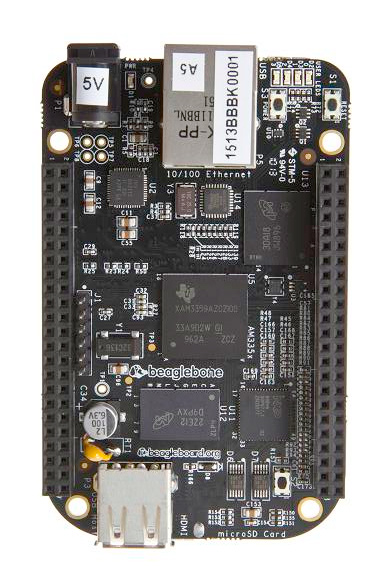
\includegraphics[width=3.5cm]{res/Beaglebone_Black.jpg}\hcite{beagleboneBlack}
	\end{center}
\end{frame}

\begin{frame}{Echtzeit}
	\begin{center}
		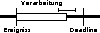
\includegraphics[width=8cm]{res/echtzeit.pdf}
	\end{center}
	\only<handout>{
		\begin{itemize}
			\item Bearbeitung ist nach einer bestimmten Zeit nach dem auftreten eines Ereignisses abgeschlossen.
			\item bei weicher Echtzeit ist dieses Verhalten wünschenswert (Video Wiedergabe)
			\item Linux ist nicht Echtzeit-Fähig
			\item Echtzeit ist oft nicht nötig
			\item Lösung ist separater uC, im SOC oder dediziertem Chip
		\end{itemize}
	}
\end{frame}
